% Created 2018-07-05 Thu 21:13
% Intended LaTeX compiler: pdflatex
\documentclass[11pt]{article}
\usepackage[utf8]{inputenc}
\usepackage[T1]{fontenc}
\usepackage{graphicx}
\usepackage{grffile}
\usepackage{longtable}
\usepackage{wrapfig}
\usepackage{rotating}
\usepackage[normalem]{ulem}
\usepackage{amsmath}
\usepackage{textcomp}
\usepackage{amssymb}
\usepackage{capt-of}
\usepackage{hyperref}
\date{\today}
\title{}
\hypersetup{
 pdfauthor={},
 pdftitle={},
 pdfkeywords={},
 pdfsubject={},
 pdfcreator={Emacs 26.0.91 (Org mode 9.1.13)}, 
 pdflang={English}}
\begin{document}

\tableofcontents

\section{Finanzmanagement}
\label{sec:orgac0718c}
Funktion des Finanzmanagement ist die zielgerichtete Gestaltung der betrieblichen Finanzwirtschaft:
\begin{itemize}
\item aktive Gestaltung der Kapitalzuführung und des Kapitalentzugs
\item eher passive Gestaltung der internen Finanzbewegungen
\item bezeichnet auch die mit den Managementaufgaben Finanzierung \& Finanzwirtschaft verantwortlich betrauten Mitglieder einer Organisation
\end{itemize}
\subsection{Finanzierung \& Wettbewerbsfähigkeit}
\label{sec:org03f0377}
Ziel der Finanzwirtschaft ist die Erreichung des finanzwirtschaftlichen Gleichgewichts
\subsubsection{Zahlungsstrom, Finanzierungsmaßnahme, Kapitalveränderung}
\label{sec:org493b0d7}
\begin{itemize}
\item \textbf{klassischer Kapitalbegriff} = Kapital ist die abstrakte Wertsumme der Bilanz; Kapital zeigt die Herkunft der Werte des Unternehmens an, unterteilt in Eigen- und Fremdkapital
\item \textbf{monetärer Kapitalbegriff} = Kapital sind im Unternehmen eingesetzte Geldmittel
\end{itemize}

Finanzwirtschaft umfasst die Kapitalbeschaffung und -verwendung der Unternehmung

\begin{enumerate}
\item Kapitalströme
\label{sec:orge449265}
\begin{figure}[htbp]
\centering
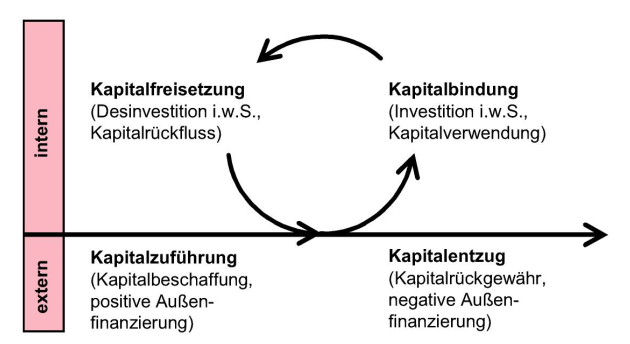
\includegraphics[width=250px]{./pictures/kapitalstroeme.png}
\caption{Kapitalveränderung als Strömungsgröße}
\end{figure} 
\begin{itemize}
\item Kapitalbindung (oder -verwendung)
\item Kapitalfreisetzung (oder -rückfluss)
\item Kapitalzuführung (oder -beschaffung)
\item Kapitalentzug (oder -abfluss)
\end{itemize}

\item Finanzielles Gleichgewicht
\label{sec:orgb14dd10}
\begin{figure}[htbp]
\centering
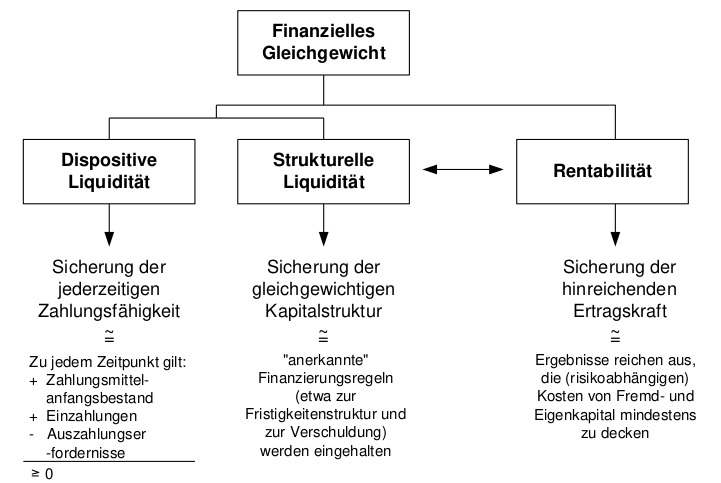
\includegraphics[width=250px]{./pictures/finanzgg.png}
\caption{Komponenten des finanziellen Gleichgewichts}
\end{figure}
\end{enumerate}
\subsubsection{Zahlungsbeziehungen, Finanzierungsform, Finanzierungsverträge}
\label{sec:org3afd6dd}
F. 13 von II\(_{\text{Finanzmanagement}}\)\(_{\text{1.pdf}}\)

\subsection{Bereitstellung finanzieller Ressourcen}
\label{sec:org83d4d78}
\subsection{Finanzierungsplanung}
\label{sec:org5c8db85}
\end{document}
